%kelompok 2
%Achmad Fatahillah(1154004)
%Ilga Anne Tri J.S(1154045)
%Maulyanda(1154008)
%Mefi Frinkazela Nikica(1154073)
%Simon Sorba Manangi(1154019)

\section{Variabel}
Pada sebagian besar bahasa pemrograman, nama suatu variabel
menjelaskan suatu nilai dengan tipe data tertentu 
dan menempati alamat memory yang pasti.
Variabel menyimpan data atau nilai yang dilakukan selama program dieksekusi,
Nilai variabel tersebut dapat diganti-ganti, namun tipe data selalu tetap.
Tidak demikian dengan python dimana tipe datanya dapat diubah-ubah
secara dinamis\cite{suparno2013komputasi}.

Variabel merupakan entitas yang memiliki nilai dan nilai tersebut berbeda satu dengan yang lain. Variabel mengalokasikan memori untuk menyimpan nilai.
Hal ini berarti ketika anda membuat variabel maka anda memesan beberapa ruang di memori. 
Variabel bisa digunakan untuk menyimpan bilangan bulat, desimal juga karakter.
Python sangat mementingkan indentasi, sehingga kita perlu melakukan indentasi secara konsisten. 
Indentitas tersebut dipermudah dengan menggunakan tombol Tab dan dimulai dari kolom pertama untuk setiap blok baru.

Variab membutuhkan pengenal atau bisa disebut dengan identifier yg didefinisikan oleh pemrograman. Tanda pengenal atau identifier memiliki aturan-aturan dalam penulisannya seperti:
1. harus diawali huruf atau di garis bawah
2. tidak menggunakan aritmatika
3. jika terdiri dari dua kata atau lebih,makan antarkatanya tidak boleh menggunakan spasi
4. tidak boleh menggunakan kata-kata yang sudah ada arti khususnya dalam bahasa Python
5. penggunaan huruf kecil dan besar harus dibedakan
6. panjanh maksimal yaitu 32 karakter

Variabel merupakan nama yang menunjukkan nilaitertentu. Dalam Pyton, untuk membentuk variabel cukup memberi nama pada nlai yang kita inginkan. Statement yang melakukan hal tersebut disebut assignment.
>>> pesan = “Hi, Apa kabar D43A”
>>> n = 19
>>> pi = 3.14159
Contoh diatas menunjukkan tiga buah assigment. Contoh pertama memberi nilai “Hi, Apa kabar D43A” pada variabel pesan, kedua memberi nilai 19 pada variabel n, dan ketiga memberi nilai 3.14159 pada variabel pi.\cite{utami2004logika}

Ada 2 cara untuk membuat variabel. Cara yang pertama yaitu variabel langsung dengan nilai disebut dengan inisialisasi. Sedangkan cara yang kedua dengan memasukkan nilai pada variabel yang biasa disebut penempatan.\cite{santoso2009bahasa}

Variabel python tidak perlu deklarasi eksplisit untuk memesan ruang memori. Deklarasi tersebut terjadi secara otomatis ketika menetapkan nilai ke variabel.
Tanda sama (=) digunakan untuk memberikan nilai pada variabel.

Operan di sebelah kiri operator =  nama dari variabel dan operan di sebelah kanan operator = nilai yang disimpan dalam variabel
Python memiliki lima tipe data standar -
Nomor
Tali
Daftar
tupel
Kamus

Variabel pada Python memiliki beberapa aturan seperti :
•	Case Sensitive : penggunaan huruf besar dan huruf kecil yang dibedakan.
•	Harus dimulai dengan underscore (_) atau huruf biasa, setelah itu dapat diikuti dengan huruf, angka atau underscore (_).
•	Tidak boleh mengandung karakter special seperti !,@,\#,\$ dan lainnya.
•	Hanya dapat menggunakan suatu variable setelah kita memberikan nilai ke dalamnya atau telah dilakukan assignment.
•	Setiap variable akan menyimpan referensi ke suatu objek dalam memory.\cite{santoso2009bahasa}

Variabel adalah sebuah nama yang selalu menunjukkan nilai tertentu. Dalam bahasa pemrograman Python, untuk membentuk sebuah variabel itu cukup hanya memberi nama pada nilai yang akan dibuat. Ini disebut dengan Assignment.
Contoh : 
>>>pesan="Halo, Semuanya"
Contoh di atas membuktikan bahwa itu adalah sebuah assignment, yang memberi kan sebuah nilai "Halo, Semuanya".\cite{Utami2004logika}

contoh lainnya:
\begin{equation}
>>> b = 2 # b bilangan bertipe integer
>>> print b
2
>>> b = b * 2.0 # Sekarang b bilangan bertipe float
>>> print b
4.0
\end{equation}

ke suatu object dalam memory. Untuk lebih jelasnya
dapat kita lihat contoh berikut ini :
\begin{equation}
>>> a = 2
>>> b = 3
>>> a,b = b,a
>>> a
3
>>> b
2
>>>
\end{equation}

Beberapa bentuk if adalah sebagai berikut :
\begin{equation}
a. if tunggal
if x == 1:
print ‘x bernilai 1’
b. if dengan else
if x == 1:
print ‘x bernilai 1’
else:
print ‘x tidak bernilai 1’
c. if dengan pilihan if lainnya
if x == 1:
print ‘x bernilai 1’
elif x == 2:
print ‘x bernilai 2’
else:
print ‘x tidak bernilai 1 atau 2’
d. if didalam if
if x == 1:
if y == 1:
print ‘x dan y bernilai 1’
\end{equation}

Tulisan b = 2 artinya kita memberi nilai pada variabel b dengan angka 2 yang bertipe integer
(bilangan bulat). Statemen berikutnya adalah melakukan operasi perkalian b ∗ 2.0 lalu hasilnya
disimpan pada variabel yang sama yaitu variabel b. Dengan demikian nilai b yang lama
akan diganti dengan nilai b yang baru, yaitu yang berasal dari operasi yang terakhir.
Sebagai Konsekuensi atau hasil dari operasi yang dirancang atau dibuat tersebut, 
sekarang variabel b memiliki tipe data float, 
suatu tipe yang berkaitan dengan bilangan pecahan atau desimal. 
Nilai variabel b menghasilkan nilai 4.0 atau empat\ref{pythonvariable}.
\begin{figure}[ht]
	\centerline{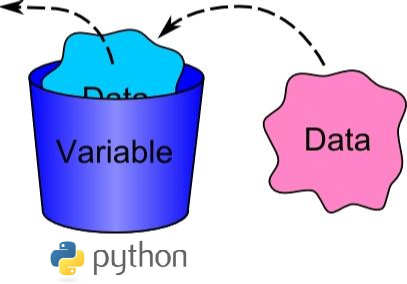
\includegraphics[width=0.25\textwidth]{figures/pythonvariable.png}
	\caption{gambar yang menggambarkan keadaan variabel pada python}
	\label{pythonvariable}
	\end{figure}

Tanda pagar (#) menyatakan awal dari suatu komentar. Komentar adalah bagian dari
script/program python yang tidak akan dieksekusi oleh interpreter. 


Python mementingkan indentasi, sehingga perlu indentasi yang konsisten. Indentasi dipermudah sesuai penggunaan
tombol Tab dan dimulai dari kolom pertama untu setiap blok baru. 

Bahasa pemrograman Python suatu fasilitas  shell di Linux, sehingga kita untuk mencoba penggunaan
Python secara leluasa. Lokasi instalan Python default pada distribusi Linux.

keunggulan Python adalah :
1. Python is powerful and fast = suatu kumpulan modul-modul yang sangat baik dan dapat menangani secara praktis setiap domain masalah
2. Python plays well with others = Python bisa berintegrasi dengan Component Object Model (COM) 
3. Python runs everywhere = versi Python berjalan di .NET, Java Virtual Machine dapat melihat bahwa sumber yang sama dapat berjalan tanpa perubahan berarti pada setiap sistem operasi tersebut.
4. Python is Open = Python dilisensi open source membuat Python digunakan dan disebarkan secara free,
5. Python is friendly and easy to learn = okumentasi yang lengkap merupakan salah satu fasilitas Python yang disenangi penggunanya. Apabila pembaca melakukan instalasi Python

Dalam menulis program, akan menggunakan code yang pernah kita  buat atau ditulis sebelumnya, pasti
kita gunakan kembali, dengan beberapa nilai berbeda.
 
Tentu saja tidak mungkin menuliskan kembali kode yang ingin dipanggil ulang tersebut.
Solusinya, supaya dapat dikelompokan kode-kode yang sering dipanggil ulang dalam suatu kelompok.

Selain itu dapat memecah masalah-masalah yang besar  menjadi masalah-masalah yang lebih kecil.
Dalam C atau bahasa pemrograman lain, biasanya digunakan istilah function.

Kemampuan python dalam mengelola tipe data sangat baik. Untuk mendeklarasikan suatu variabel dilakukan secara langsung tanpa menyebutkan tipe datanya, ini yang membedakan python dengan bahasa lain. Python akan menentukan tipe datanya secara otomatis. Python juga mendukung konversi dan perhitungan antar tipe data dengan ketelitian yang tinggi. Python membagi tipe data ke dalam 2 jenis bilangan (semua tipe yang berhubungan dengan angka murni) dan string. Untuk tipe data dalam rumpun bilangan termasuk didalamnya adalah integer, long, float, oktal, hexadimal dan bilangan kompleks. Hal-hal yang harus diperhatikan :
•	Untuk bilangan oktal dan hexa masing-masing diawali dengan 0 dan 0x
•	Untuk bilangan panjang diakhiri menggunakan karakter l atau L
•	Untuk bilangan float, gunakan e atau E pada eksponensial
•	Untuk bilangan kompleks dibagi ke menjadi bagian real dan imajiner, dan diakhiri dengan j atau J Operator untuk tipe dalam rumpun bilangan.\cite{utamipemrograman}

\subsection{Membuat Variabel}
Variabel atau peubah memiliki pengertian sembarang symbol yang dapat dimuati oleh sembarang himpunan bilangan. Dalam pengertian komputasi sebuah nama yang digunakan untuk menyimpan nilai dengan kapasitas tertentu dan alamat tertentu dalam memori komputer. Variabel merupakan pendaftaran tipe data bagi variabel, konstanta dan parameter yang digunakan sebuah program agar mempunyai alamat penyimpanan dan kapasitas data dalam memori komputer. Dalam membuat variabel hindari spasi dan menggunakan karakter khusus, selain itu juga nama dalam kata cadangan Python (seperti input, eval, if, elif, for, def, dan lain-lain) tidak dapat menjadi variabel.\cite{irfani2016bahan}

Nama variabel atau disebut juga dengan identifier dalam bahasa pemrograman Python juga dapat berupa kumpulan dari huru (letter) maupun angka (digit) yang dengan cara membedakan huruf kecil dan juga huruf besar, Karakter pertama pada identifier harus berupa huruf dan juga perlu diketahui bahwa penggunaan karakter garis bwah itu juga dapat digunakan.
Kesalahan sintax akan muncul apabila dalam penamaan sebuah variabel itu tidak sesuai dengan aturan yang ada.
Contoh :
>>>876swafm="Radio Swa"
SyntaxError: invalid syntax
>>>more$=1000000
SyntaxError: invalid syntax
Baris pertama itu salah, karena pada 876swafm karakter pertamanya itu bukanlah huruf. Pada baris ketiga juga salah karena pada more$ berisi karakter dolar.

Tidak seperti pemrograman pada lainnya, variabel pada Python tidak harus dideklarasikan secara eksplisit. Pendeklarasian variabel terjadi secara otomatis ketika kita memberikan sebuah nilai pada suatu variabel. Tanda sama-dengan (=) digunakan untuk memberikan nilai pada suatu variabel. Operan di sebelah kiri dari tanda (=) adalah nama variabel, sedangkan operan yang sebelah kanan dari tanda (=) adalah nilai yang diberikan pada variabel.\cite{utamipemrograman}

\begin{equation}
>>>harga = 100
>>>diskon = 25
>>>harga - diskon
75
\end{equation}

Pada contoh di atas, 100 dan 25 merupakan nilai yang diberikan pada variabel harga dan diskon. Sedangkan pernyataan harga-diskon akan menghitung selisih antara harga dengan diskon. Variabel juga dapat menyimpan suatu nilai berupa teks (dibaca string).

\begin{equation}
>>>a = 'sekolah'
>>>b = 'dasar'
>>>a + b
'sekolahdasar'
\end{equation}

Variabel juga dapat menyimpan dua nilai string atau lebih dengan menggunakan operator (+).

\begin{equation}
>>>c = 'Py' + 'thon'
>>>c
'Python'
\end{equation}

Jika kita telah memberikan nilai pada variabel, kita dapat menggunakan variabel tersebut pada yang lainnya.

\begin{equation}
>>>a = 2
>>>a = a + 3
>>>a
5
\end{equation}

Selain itu, juga dapat memberikan sebuah nilai untuk beberapa variabel.

\begin{equation}
>>>p=q=r=1
>>>p
1
>>>q
1
>>>r
1
\end{equation}

Selain itu, kita dapat memberikan beberapa nilai untuk beberapa variabel (disebut multiple assignment).

\begin{equation}
>>>x, y, z = 1, 2, 'belajar Python'
>>>x
1
>>>y
2
>>>z
'belajar Python'
\end{equation}

Bentuk lain dari contoh di atas, kita bisa menggunakan tanda kurung-buka kurung-tutup.

\begin{equation}
>>>(x, y, z) = (1, 2, 'belajar Python')
Cara di atas, dapat juga kita gunakan untuk pertukaran nilai variabel.
>>>(x, y) = (10, 20)
>>>x
10
>>>y
20
>>>(x, y) = (y, x)
>>>x
20
>>>y
10
\end{equation}

Contoh-contoh  pada prompt Python adalah sebagai berikut 

\begin{equation}
>>> a = 1
>>> a
1
>>> b = 2
>>> b
2
>>> c = a + b
>>> c
3
>>> d = a - b
>>> d
-1
>>> print ‘Nilai d adalah : ‘, d
Nilai d adalah : -1
>>> print ‘Nilai c adalah : ‘, c
Nilai c adalah : 3
>>> e
Traceback (most recent call last):
File “<stdin>”, line 1, in ?
\end{equation}

\subsection{Aturan Penulisan Variabel}
• Nama variabel boleh diawali menggunakan huruf atau garis bawah (_), contoh: nama, _nama, namaKu, nama_variabel.
• Karakter selanjutnya dapat berupa huruf, garis bawah (_) atau angka, contoh: __nama, n2, nilai1.
• Karakter pada nama variabel bersifat sensitif (case-sensitif). Artinya huruf besar dan kecil dibedakan. Misalnya, variabel_Ku 	   dan variabel_ku, keduanya adalah variabel yang berbeda.
• Nama variabel tidak boleh menggunakan kata kunci yang sudah ada dalam python seperti if, while, for, dsb.

\subsection{Menghapus Variabel}
Ketika sebuah variabel tidak dibutuhkan lagi, maka kita bisa menghapusnya dengan fungsi del().
Contoh:

\begin{equation}
>>> nama = "petanikode"
>>> print nama
petanikode
>>> del(nama)
>>> print nama
Traceback (most recent call last):
  File "<stdin>", line 1, in <module>
NameError: name 'nama' is not defined
>>>
\end{equation}

Pada perintah terakhir, kita akan mandapatkan NameError. Artinya variabel tidak ada di dalam memori alias sudah dihapus.

\subsubsection{Penempatan variable pada yang semestinya}
Misalkan sebuah data pribadi berisi nama, alamat, umur, tempat lahir, tanggal lahir, indeks prestasi kumulatif akan memberikan 6 (enam) buah variabel dengan tipe datanya.
\begin{figure}[ht]
	\centerline{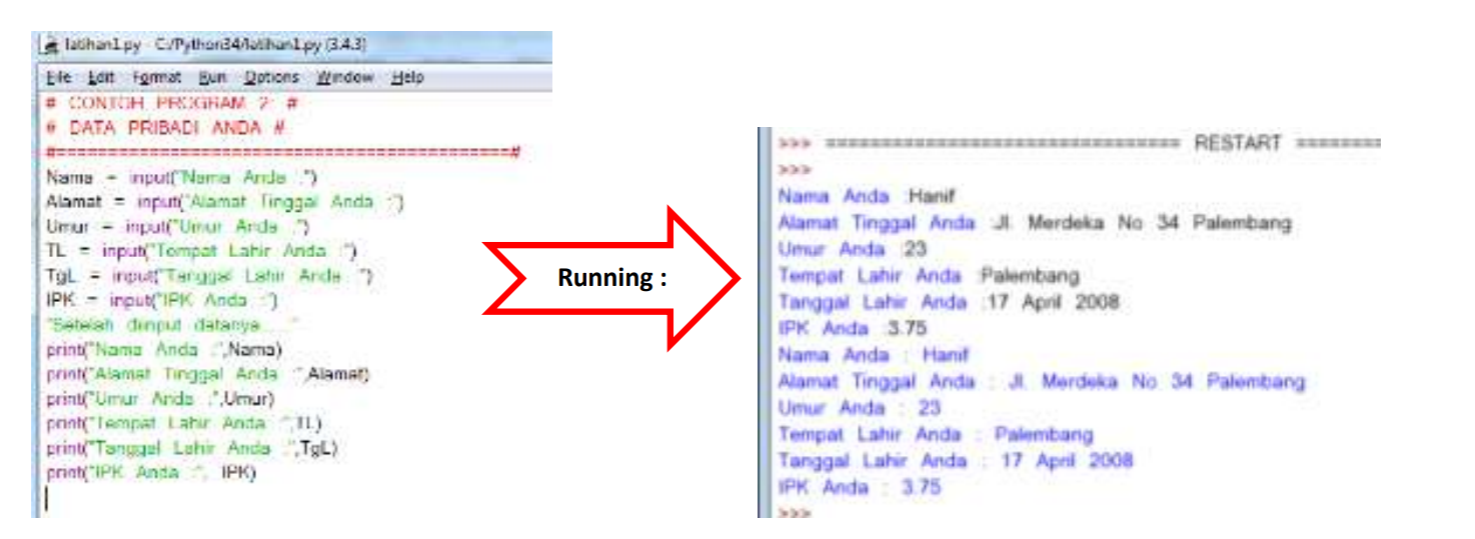
\includegraphics[width=1\textwidth]{figures/tipedatastring.png}}
	\caption{Tampilan Contoh Input/Output Tipe Data String}
	\label{tipedatastring}
	\end{figure}

\begin{figure}[ht]
	\centerline{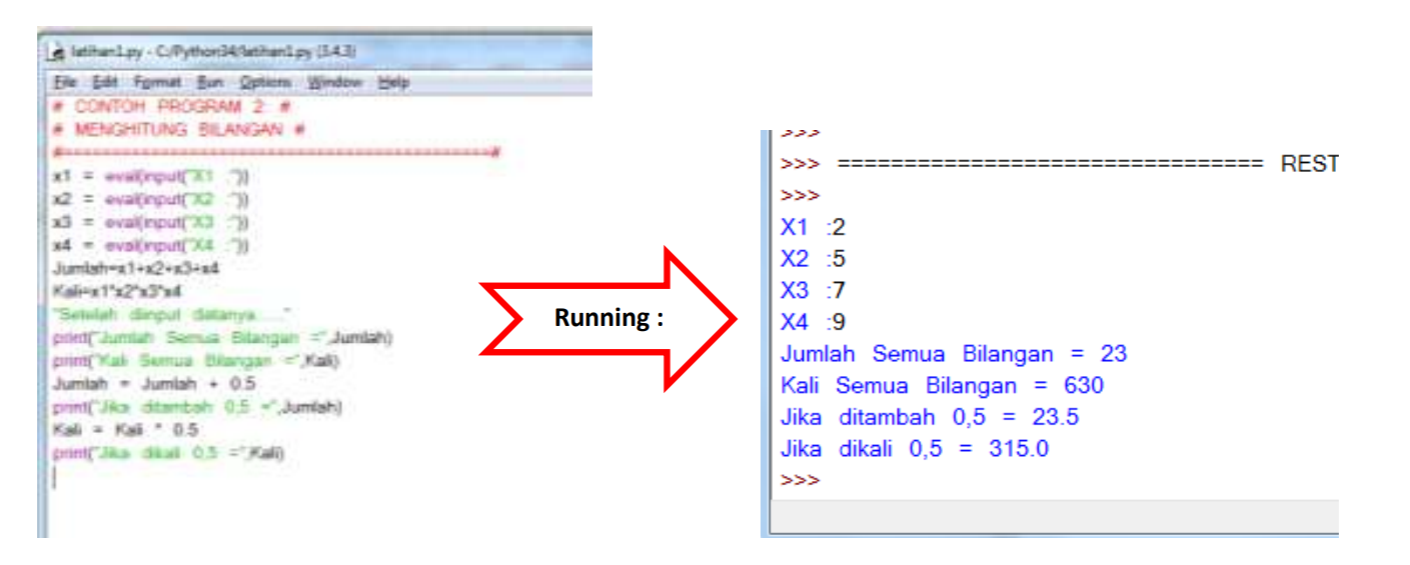
\includegraphics[width=1\textwidth]{figures/tipedatabilangan.png}}
	\caption{Tampilan Contoh Input/ Output Tipe Data Bilangan}
	\label{tipedatabilangan}
	\end{figure}

Pada Gambar 2.2 \ref{tipedatabilangan} terlihat input/output pada tipe data bilangan dengan hasil yang berbeda tipe bilangannya yaitu tipe integer (bilangan bulat) atau float (bilangan berkoma).\cite{irfani2016bahan}

\subsusection{Memberikan nilai ke dalam variable}
Lakukan inisiasi variabel atau konstanta dari permasalahan berikut! Menjumlahkan hasil dari total harga pada saat konsumen membeli beberapa barang.

Langkah 1: Inisiasi Persoalan 
Variabel/ konstanta input :  
kode_barang, nama_barang, harga_satuan_barang, 
jumlah_per_barang_beli, total_harga_per_transaksi = 0 
Proses :  harga_beli_per_barang = harga_satuan_barang * jumlah_per_barang_beli 
total_harga_per_transaksi=harga_beli_per_barang + total_harga_per_transaksi
Output :  total_harga_per_transaksi

Langkah 2: Menetapkan Tipe Data 
kd_brg, nama_brg bertipe data string 
jum_brg bertipe data integer harga_satuan, harga_beli, total_hrg_brg bertipe data float 

Langkah 3 : Kode program
\begin{figure}[ht]
	\centerline{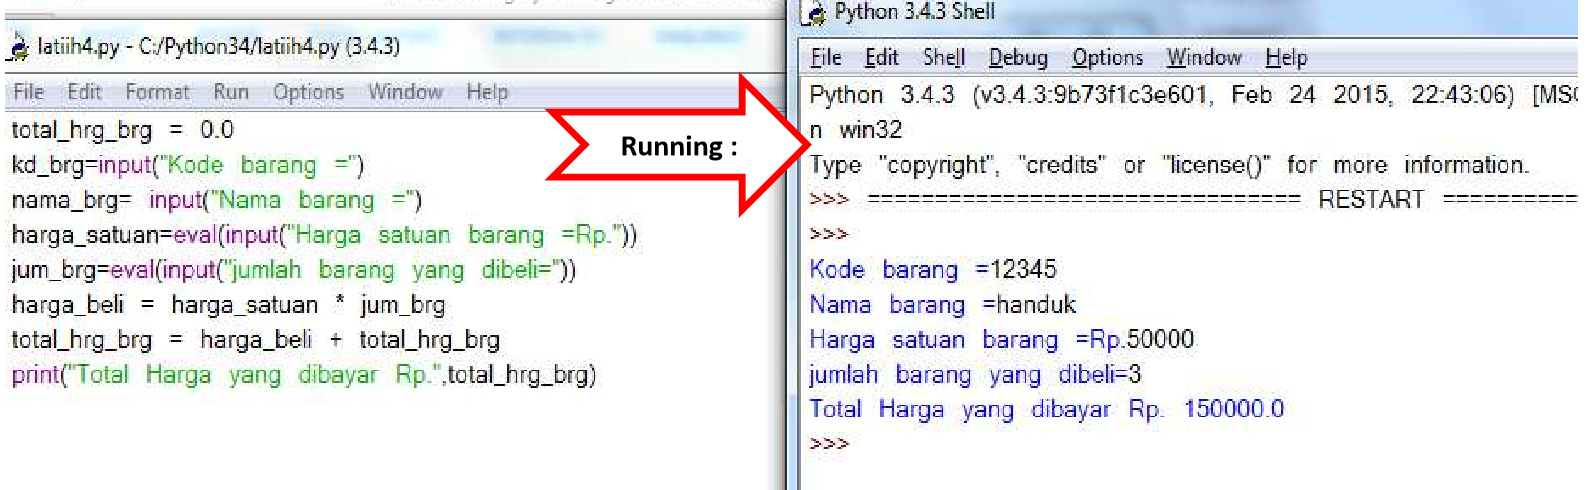
\includegraphics[width=0.50\textwidth]{figures/code.png}
	\caption{kode program}
	\label{code}
	\end{figure}
  
\subsubsection{Mencetak nilai dalam variable} 
Mencetak nilai dalam sebuah variabel menggunakan pernyataan print, perhatikan 
contoh berikut ini. 
\begin{figure}[ht]
	\centerline{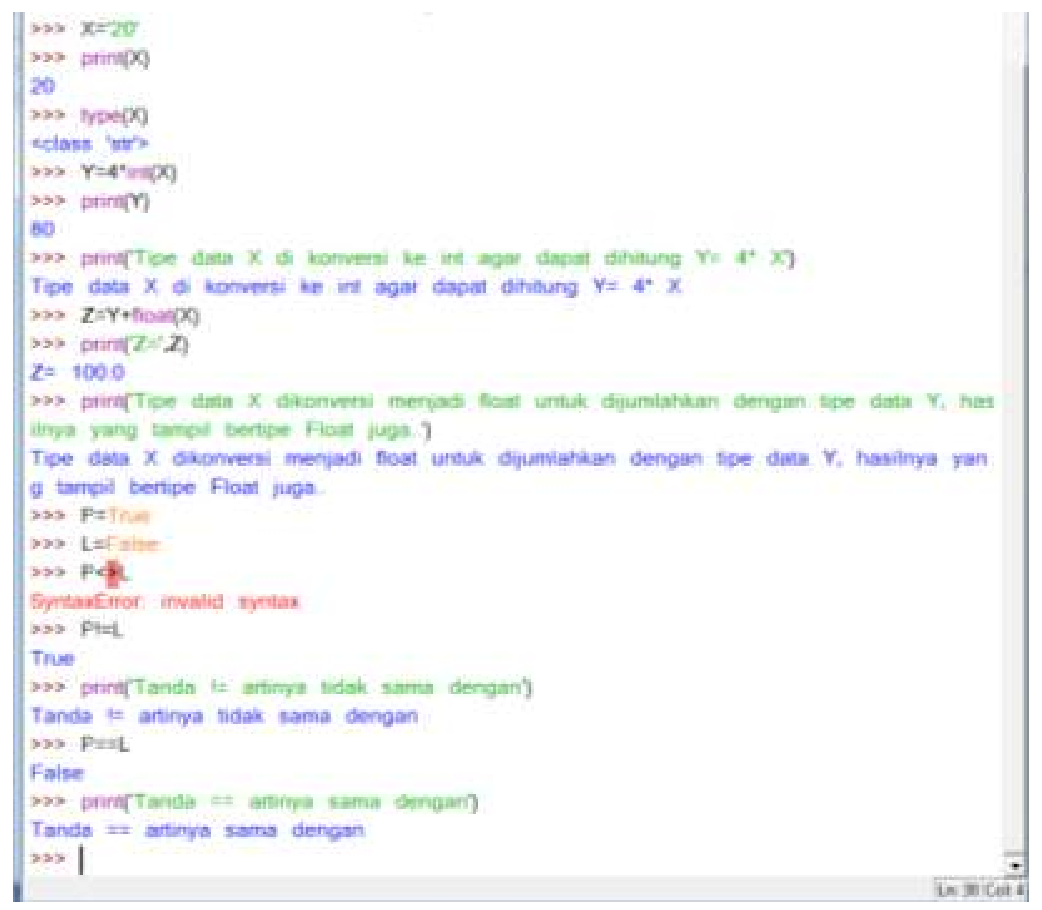
\includegraphics[width=0.25\textwidth]{figures/konversi.png}
	\caption{Tampilan Contoh Konversi Tipe Data String dan Integer}
	\label{Tipe Data String dan Integer}
	\end{figure}

\subsection{Bilangan integer dan float}
Seperti telah disinggung bahwa python mengenal bilangan bertipe integer dan float. 
Perbedaan tipe bilangan ini bisa jadi berpotensi menimbulkan masalah. 
Ini contohnya
\begin{equation}
>>> 1/2 # bilangan integer dibagi bilangan integer
0 # tentu saja ini keliru, mestinya 0.5
>>> 1/2.0 # bilangan integer dibagi bilangan float
0.5 # kali ini hasilnya tepat
\end{equation}


\subsection{List}
List adalah sejumlah object yang dipisahkan oleh tanda koma (,) dan diapit oleh kurung siku
([ ]). Begini contohnya:
\begin{equation}
>>> a = [1.0, 2.0, 3.0] # cara membuat list
>>> a.append(4.0) # tambahkan 4.0 kedalam list
>>> print a
[1.0, 2.0, 3.0, 4.0]
>>> a.insert(0,0.0) # sisipkan 0.0 pada posisi 0
>>> print a
[0.0, 1.0, 2.0, 3.0, 4.0]
>>> print len(a) # menentukan panjang list
5
\end{equation}
Jika kita memberikan statemen b = a, maka itu tidak berarti bahwa variabel b terpisah dengan
variabel a. Di python, statemen seperti itu diartikan hanya sebagai pemberian nama lain
(alias) kepada variabel a. Artinya, perubahan yang terjadi baik itu di a ataupun di b, maka hasil
akhir mereka berdua akan sama saja. Setiap perubahan yang terjadi di b akan berdampak di a.
Untuk meng-copy a secara independen, gunakan statemen c = a[:]. 
Berikut adalah beberapa contoh lambang atau tanda untuk melengkapi setiap statement pada
variabel yang ada\ref{operate}.
\begin{figure}[ht]
	\centerline{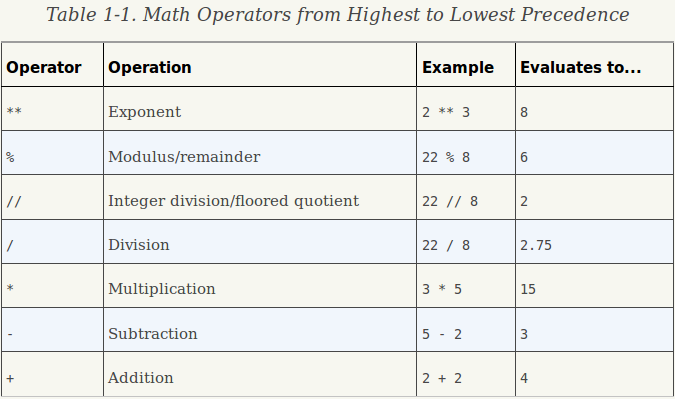
\includegraphics[width=0.25\textwidth]{figures/operate.png}
	\caption{gambar tanda operasi pada python}
	\label{operate}
	\end{figure}





